%\documentclass[conference]{IEEEtran}
\documentclass{sig-alternate-10pt}

\usepackage[latin1]{inputenc}
\usepackage[T1]{fontenc}
\usepackage[norsk, english]{babel}
\usepackage{epsfig, times}
\usepackage{longtable}
\usepackage{fancyhdr}
\usepackage{amsmath}
\usepackage{verbatim}
\usepackage{cite}
\usepackage{textcomp}
\usepackage{graphics}
\usepackage{subfigure}
\usepackage{algorithm}
\usepackage{algorithmic}
\usepackage{wrapfig}
\usepackage{url}
\usepackage{ulem}
\usepackage{color,soul}
\usepackage{graphicx}

\normalem

\newcommand\PH[1]{\textcolor{blue}{(PH: \it #1)}}
\newcommand\AP[1]{\textcolor{red}{(AP: \it #1)}}
\newcommand\HKS[1]{\textcolor{green}{(\it #1)}}

\begin{document}

%\title{Game server architectures for parallel execution and scalability}
\title{LEARS: A Lockless, Relaxed Atomicity State Model for Parallel Execution in Game Servers}

\author{
  \large
  Kjetil Raaen, H{\aa}vard Espeland, H{\aa}kon K. Stensland,
  Andreas Petlund, P{\aa}l Halvorsen, Carsten Griwodz\\
  \large
  NITH, Norway \ \ \ \ Simula Research Laboratory, Norway \ \ \ \ 
  IFI, University of Oslo, Norway\\
  \large
  Email: raakje@nith.no, \{haavares, haakonks, apetlund, paalh, griff\}@ifi.uio.no
}


%\date{\today}
\maketitle

\begin{abstract}
Supporting thousands of interacting players in a virtual world poses
huge challenges with respect to processing. To host as many
players as possible, the server software has
to implement support for massive parallelism. Earlier work within the
field suggests that this is difficult due to synchronization issues, but
in this paper, we present the design and implementation of a game server
architecture based on a model that allows for massive parallelism.
%The server design is evaluated using
%replayed traces from actual gameplay to create server traffic. 
%We also discuss challenges that arise as different
%dependency requirements are introduced to the system. 
Our prototype is evaluated using traces from live game sessions where
we measure the server response time for all objects that need timely
updates. We also measure how the response time for the multi-threaded
implementation varies with the number of threads used. Our results
show that the challenge of scaling up a game-server can be an
embarrassingly parallel problem.
\end{abstract}

\section{Introduction}

%Over the last decade, online multi-player gaming has experienced an
%amazing growth. Providers of the popular online games must deliver a
%reliable service to thousands of concurrent players meeting strict
%processing deadlines in order for the players to have an acceptable
%quality of experience (QoE). 

%% Game types and server architectures
%% Game server architecture models.
%% -FPS, RTS and small, local servers with low pings.
%% -Separated gameworld instances, each with < 1000 players
%% -Shards, grids and area of interest.

%% Game designs that allow thousands of players to interact in a small
%% space is also challenging.

One major goal for large game providers is to support as many
concurrent players in a game-world as possible while preserving the
strict latency requirements in order for the players to have an
acceptable quality of experience (QoE). In order to achieve this,
game-worlds are typically partitioned into areas-of-interest to
minimize message passing between players with no interaction and to
allow the game-world to be divided between servers. This approach is
however limited by the distribution of players in the game-world, and
the problem is that the distribution of players is heavy-tailed with
about 30\% of players in 1\% of the game area~\cite{chen-2006}. 

In such scenarios, the important metric for online multi-player games
is latency. Claypool et. al.~\cite{claypool++-2006} classify different
types of games and conclude that for first person shooter (FPS) and
racing games, the threshold for an acceptable latency is 100ms. For
other classes of networked games, like real-time strategy (RTS) and
massively multi-player online games (MMOGs) players will tolerate
somewhat higher delays, but there are still strict latency
requirements in order to provide a good QoE. The accumulated latency
of network transmission, server processing and client processing adds
up to the latencies that the user is experiencing, and reducing any of
these latencies will improve the user's experience.

%There is a prevailing belief in the need for single threaded execution
%of the game event loop in order to preserve what is seen as critical
%dependencies in the game~\cite{Abdelkhalek2004++} \PH{Har vi noen
%  eksempler her som bruker dette??}. Due to this
%constriction, even when provisioning for scalability in designing an
%online game, service providers still find that the processing power on
%the server side is becoming scarce~\cite{Cai2002++}.
%\PH{Kan vi omformulere dette? \cite{Cai2002++} er eldre enn %~\cite{Abdelkhalek2004++}}
The traditional design of massively multi-player game servers rely \textit{sharding} for scalability beyond what a single CPU core can handle. \textit{Sharding} involves making a new copy of an area of a game, where players in different copies are unable to interact. This approach eliminates most requirements for communication between the processes running individual shards. An example of such a design can be found in~\cite{chu-2008}.

The industry is now experimenting with
implementations that allow for a greater level of
parallelization. One known example is Eve Online \cite{drain-2008}. With LEARS, we
take this approach even further and focus on how many players can be
handled in a single segment of the game world. We present a model that
allows for better resource utilization of multi-processor, game server
systems which should not replace spatial partitioning techniques for
work distribution, but rather complement them to improve on their
limitations. Furthermore, a real prototype game is used for evaluation
where captured traces are used to generate server load. We compare
multi-threaded and single-threaded implementations in order to measure
the overhead of parallelizing the implementation and showing the
experienced benefits of parallelization. The change in responsiveness
of different implementations with increased load on the server is
studied, and we discuss generic elements of this game design which
impact of our chosen platform of implementation.

Our results indicate that it is possible to design an ``embarrassingly
parallel'' game server. We also observe that the implementation is
able to handle a quadratic increase of in-server communication when
many players interact in a game-world hotspot.


\section{LEARS: The Basic Idea}\label{sec:concept}
Traditionally, game servers have been implemented much like game
clients. They are based around a main loop, which updates every active
element in the game. These elements include for example player
characters, non-player characters and projectiles. The simulated world
has a list of all the active elements in the game and typically calls
an ``update'' method on each element. The simulated time is kept
constant throughout each iteration of the loop, so that all elements get updates at the same points in simulated time. This point in
time is referred to as a \textit{tick}.  Using this method, the active
element performs all its actions for the tick. Since only one
element updates at a time, all actions can be performed directly. The
character reads input from the network, performs updates on itself
according to the input, and updates other elements with the results of
its actions.

%
%To make a parallel game server with minimal locking, the system needs
%to be designed from the ground up with parallelism in mind.
LEARS is a game server model with support for lockless, relaxed-atomicity
state-parallel execution.  The main concept is to split the
game server executable into lightweight threads at the finest possible
granularity. Each update of every player character, AI opponent and
projectile runs as an independent work unit. 
%Using this approach, the
%theoretical parallelism is proportional to the load on the
%server \CG{(I don't get it?)}. To do this \CG{(you don't mention before that
%you're doing anything)}, we must relax the presumed deterministic
%requirements of a game server, and we \CG{\sout{will}} show that this approach
%retains consistency and is applicable to real-world games.
%
%\CG{(That sounds too fluffy for me. Shouldn't the argument be somewhat more
%concrete, similar to this:
%The cycles in a highly
%interactive, multiuser game are rather short, so short actually that
%client-server latency differences between players are so large compared
%to the cycle length that the order of events as they are generated by the
%client is irrelevant. Similarly, the order of arrival of these events at
%the server becomes irrelevant because of these differences. If we can
%assume that every cycle can be considered an atomic tick, then state can
%actually be double-buffering between cycles. Processing an event does then
%require reading state from the previous cycle, processing independently
%from all other input events, and writing to the new cycle. If the writing
%destinations are distinct, locking becomes unnecessary.'')}

White et al.~\cite{white++2008} describe a model they call a 
\textit{state-effect pattern}. Based on the observation that changes in a large, actor-based simulation are happening \textit{simultaneously}, they separate read and write operations. Read operations work on a consistent previous state, and all write operations are batched and executed to produce the state for the next tick. This means that the ordering of events scheduled to execute at a tick does not need to be considered or enforced. 
For the design in this paper, we additionally remove the requirement for batching of write operations, allowing these to happen anytime during the tick. The rationale for this relaxation is found in the way traditional game servers work. In the traditional single-threaded main-loop approach, every update is allowed to change any part of the simulation state at any time. In such a scenario the state at a given time is a combination of values from two different points in time, current and previous, exactly the same situation that occurs in the design presented here.
%
%This is the case for many
%games and is mainly an issue of game design, i.e., what is the desired
%behavior if two players perform conflicting
%actions at the same instant. In the
%traditional main-loop approach, every event in a
%game scheduled for a tick are executed by the main loop. The
%main loop process these in arrival order. Thus, the ordering is highly
%influenced by the client latencies and at which point in time between
%two ticks the event was dispatched by the
%client. Remember that a tick is the smallest amount of time
%considered by the game, and this means there is no correct order to
%execute conflicting events within a single tick. As such, the
%ordering of events scheduled for a tick in a traditional main
%loop is \textit{not} deterministic. LEARS takes advantage of this
%relaxation and allows events scheduled
%for a tick to execute in any order.

The second relaxation relates to the atomicity of game state updates. The fine
granularity creates a need for significant communication between threads
to avoid problematic lock contentions. Systems where
%
elements can only update their own state and read any state
without locking~\cite{Abdelkhalek2004++}
%
do obviously not work in all cases. However, game servers are not
accurate simulators, and again, depending on the game design, some
(internal) errors are acceptable without violating game state
consistency. 
Consider
the following example: Character A moves while character B attacks. If
only the X coordinate of character A is updated at the point in time
when the attack is executed, the attack sees character A at a position with the new X coordinate and the old Y coordinate.  This position is within the accuracy of the
simulation which in any case is no better than the distance an object
can move within one tick. 

On the other hand, for actions where a margin of error is not
acceptable, transactions can be used keeping the object's state
internally consistent. However, locking the state is
expensive. Fortunately, most common game actions do not require
transactions, an observation that we take advantage of in LEARS.
%but if two variables in an object's game state must be
%altered simultaneously to retain consistency, locking must be used.

These two relaxations allow actions to be performed on game objects in
any order without global locking. It can be implemented using message
passing between threads and retains consistency for most game actions.
This includes actions such as moving, shooting, spells and so forth.
Consider player A shooting at player B: A subtracts her ammunition state, and
send bullets in B's general direction by spawning bullet objects. The
bullet objects runs as independent work units, and if one of them hits player B, it
sends a message to player B. When reading this message, player B
subtracts his health and sends a message to player A if it reaches zero.
Player A then updates her statistics when she receives player B's message. This series of events can be time critical at certain points. The most important point is where the decision is made if the bullet hits player B. If player B is moving, the order of updates can be critical in deciding if the bullet hits or misses. In the case where the bullet moves first, the player does not get a chance to move out of the way. This inconsistency is however not a product of the LEARS approach. Game servers in general insert active items into their loops in an arbitrary fashion, and there is no rule to state which order is ``correct''.

The end result of our proposed design philosophy is that there is no
synchronization in the server under normal running conditions. Since
there are cases where transactions are required, they can be implemented
outside the LEARS event handler running as transactions
requiring locking. In the rest of the paper, we consider a
practical implementation of LEARS, and evaluate its performance and
scalability.

\section{Design and Implementation}\label{sec:implementation}

%%\PH{A detailed description of your parallel thread-pool based
%%  server. Point out the differences to the event-loop-based solution,
%%  and of course all the nice things like no locking etc.. What do you
%%  avoid wrt. the problem in traditional designs like dependencies, If
%%  possible, generalize the concepts from the Java-specific
%%  implementation. Are there any design/implementation specific
%%  alternatives that should be discussed. Also describe the example
%%  game and tell why this is a representative example in order to
%%  indicate that the results/conclusions are valid beyond the case
%%  study. \\ Screenshots?  Overview figure of the architecture? }

In our experimental prototype implementation of the LEARS concept, the
parallel approach is realized using thread pools and blocking queues.

\subsection{Thread pool}

Creation and deletion of threads incur large overheads,
and context switching is an expensive operation.  These overheads
constrain how a system can be designed, i.e., threads should be kept
as long as possible, and the number of threads should not grow
unbounded. We use a \textit{thread pool} pattern to work around these
constraints, and a thread pool executor (the Java
\texttt{ThreadPoolExecutor} class) to maintain the pool
of threads and a queue of tasks. When a thread is available, the
executor will pick a task from the queue and execute it. The thread
pool system itself is not preemptive, so the thread will run each task
until it is done. This means that in contrast to normal threading,
each task should be as small as possible, i.e., larger units of work should
be split up into several sub-tasks.

The thread pool is a good way to balance the number of threads
when the work is split into extremely small units. When an active
element is created in the virtual world, it will be scheduled for
execution by the thread pool executor, and the active element will
update its state exactly as in the single threaded case.
%
Furthermore, our thread pool supports the concept of delayed
execution. This means that tasks can be put into the work queue for
execution at a time specified in the future.
%
When the task is finished for one time slot, it can reschedule itself
for the next slot, delayed by a specified time. This allows active
elements to have any lifetime from one-shot executions to the duration
of the program. It also allows different elements to be updated at
different rates depending on the requirements of the game developer.

\subsection{Blocking queues}

The thread pool executor used as described above will not constrain
which tasks are executed in parallel. All systems elements
must therefore allow any of the other elements to execute concurrently. 

To enable a fast communication between threads with shared memory (and
caches), we use \textit{blocking queues}, using the Java
\texttt{Blocking\-Queue} class, which implements queues that are
synchronized separately at each end. This means that elements can be
removed from and added to the queue simultaneously, and since each of
these operations are extremely fast, the probability of blocking is
low.
%
Thus, these queues allow information to be passed
between active objects. Each active object that can be influenced by
others has a blocking queue of messages. During its update, it will
read and process the pending messages from its queue. Other active
elements put messages in the queue to be processed when they need to
change the state of other elements in the game.

%This form of communication is extremely fast. As all threads share the
%same memory, trasfer through memory. Data can even be transfered
%without leaving cache.
\vspace{4mm}
\subsection{Our implementation}
% Also describe the example
% game and tell why this is a representative example in order to
% indicate that the results/conclusions are valid beyond the case
% study.
 
To demonstrate LEARS, we have implemented a prototype
game containing all the basic elements of a full MMOG with the
exception of persistent state.
%
Persistent state do introduce some complications, but as database
transactions are often not time critical and can usually be scheduled
outside peak load situations, we leave this to future work.

\begin{figure}
\centering
%\vspace{-3mm}
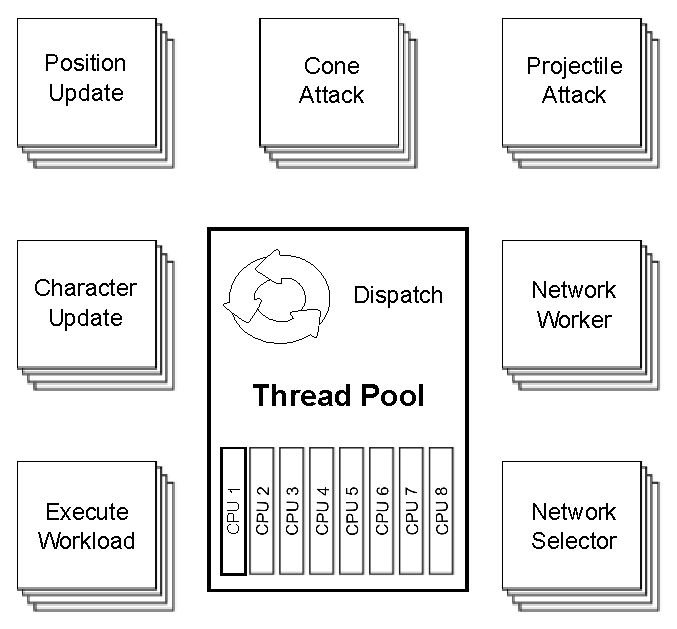
\psfig{file=FIG/server.eps,width=7cm}
\vspace{-3mm}
\caption{Design of the Game Server}
\vspace{-3mm}
\label{fig:server}
\end{figure}

\begin{wrapfigure}{r}{4.5cm}
  \vspace{-2mm}
  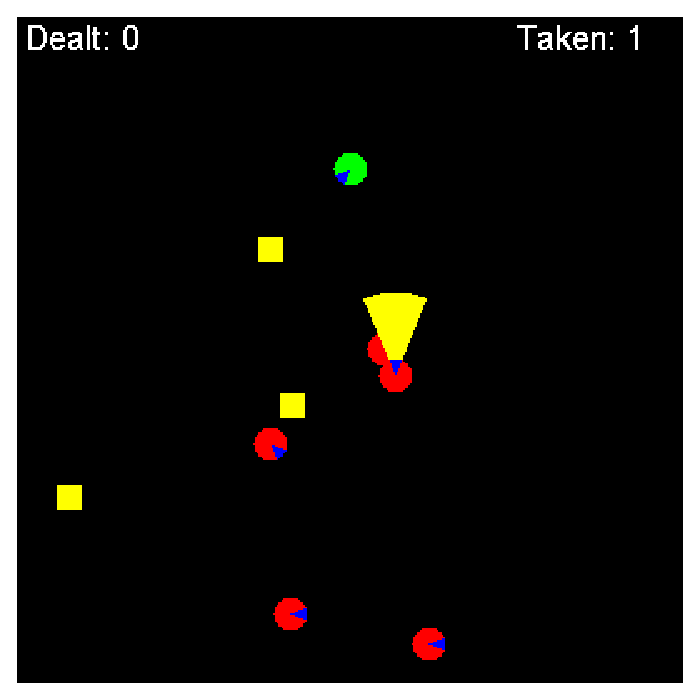
\includegraphics[width=4.5cm]{FIG/screenshot}
  \caption{Screen shot of a game with six players.}
  \vspace{-2mm}
  \label{fig:screen}
\end{wrapfigure}

In the game, each player controls a small circle ("the
character") with an indicator for which direction they are heading
(see figure~\ref{fig:screen}). The
characters are moved around by pressing keyboard buttons. They also
have two types of attack, i.e.,  one projectile and one instant area of effect
attack. Both attacks are aimed straight ahead. If an attack hits
another player character, the attacker gets a positive point, and the
character that was hit gets a negative point. The game
provides examples of all the elements of the design described
above:
\begin{itemize}
\item The player character is a long lifetime active object. It
  processes messages from clients, updates states and potentially
  produces other active objects (attacks). In addition to position,
  which all objects have, the player also has information about how
  many times it has been hit and how many times it has hit others. The
  player character also has a message queue to receive messages from
  other active objects. At the end of its update, it will enqueue
  itself for the next update unless the client it represents has
  disconnected.
\item The frontal cone attack is a one shot task that finds player
  characters in its designated area and sends messages to those hit so
  they can update their counters, as well as back to the attacking
  player informing about how many were hit.
\item The projectile is a short lifetime object that moves in the
  world, checks if it has hit anything and reschedules itself for
  another update, unless it has hit something or ran to the end of its
  range. The projectile can only hit one target.
\end{itemize}

%\begin{figure}[h]
%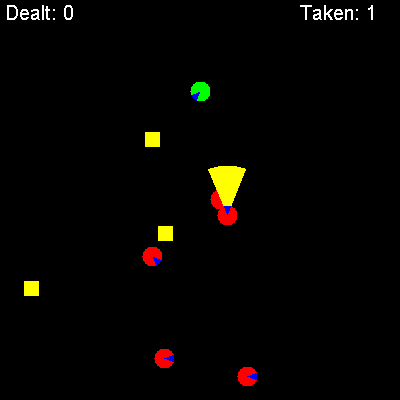
\includegraphics[width=1.0\linewidth, bb=0 0 400 400]{FIG/screenshot.png}
%\caption{Screenshot of the game with six players.}
%\end{figure}

%% \begin{figure}
%% \centering
%% %\vspace{-3mm}
%% 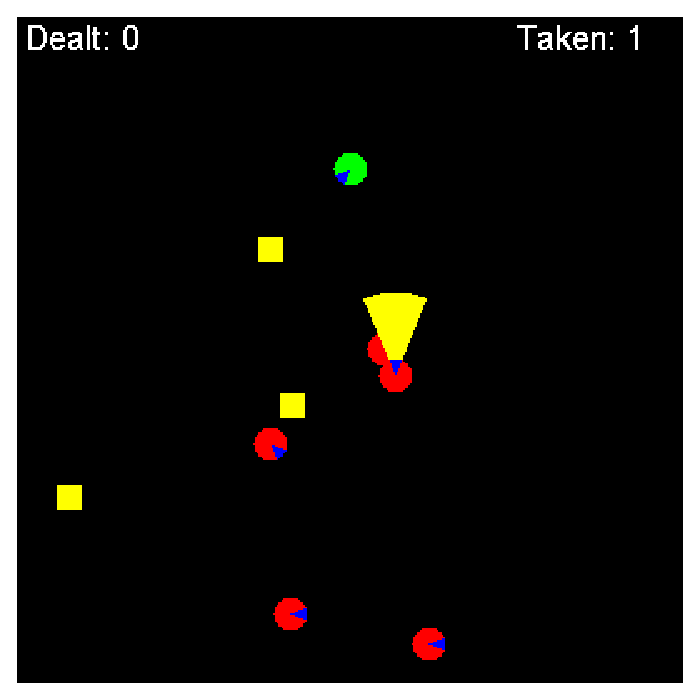
\psfig{file=FIG/screenshot.eps,width=4cm}
%% \vspace{-3mm}
%% \caption{Screenshot of game with six players.}
%% \vspace{-3mm}
%% \label{fig:screen}
%% \end{figure}

To simulate an MMORPG workload that grow linearly with number of
players, especially collision checks with the ground and other static
objects, we have included a synthetic load which emulates collision
detection with a high-resolution terrain mesh. The synthetic load
ensures that the cache is regularly flushed
%an array of floating
%point values represents a part of the gameworld. For each scheduled
%update, each character has to perform a square operation on a given
%number of elements in the array. The operation is seeded with a
%randomly generated value in order to avoid runtime optimizations in
%the virtual machine. Which elements are processed depends on the
%player's position in the gameworld. How many array elements are
%processed determines the severity of the load. By adding the synthetic
%load, the cache is dirtied 
to enhance the realism of our game server prototype compared to a
large-scale game server.
%For our experiments, 1000
%array elements were processed for each character update, emulating
%collision detection with a high-resolution terrain mesh.

The system described in this paper is implemented in Java. This
programming language has strong support for multi-threading and has
well-tested implementations of all the required components. The
absolute values resulting from these experiments depend strongly on
the complexity of the game, as a more complex game would require more
processing. In addition, the absolute values will depend on the runtime
environment, especially the server hardware, and the choice of programming
language also influence absolute results from the
experiments. However, the focus of this paper is the relative results,
as we are interested in comparing scalability of the multi-threaded
solution with a single-threaded approach and whether the
multi-threaded implementation can handle the quadratic increase in
traffic as new players join.

\section{Evaluation}\label{sec:eval}

%\subsection {Experiment setup}
%\label{sec:experiment}
%% \begin{figure}[h]
%%   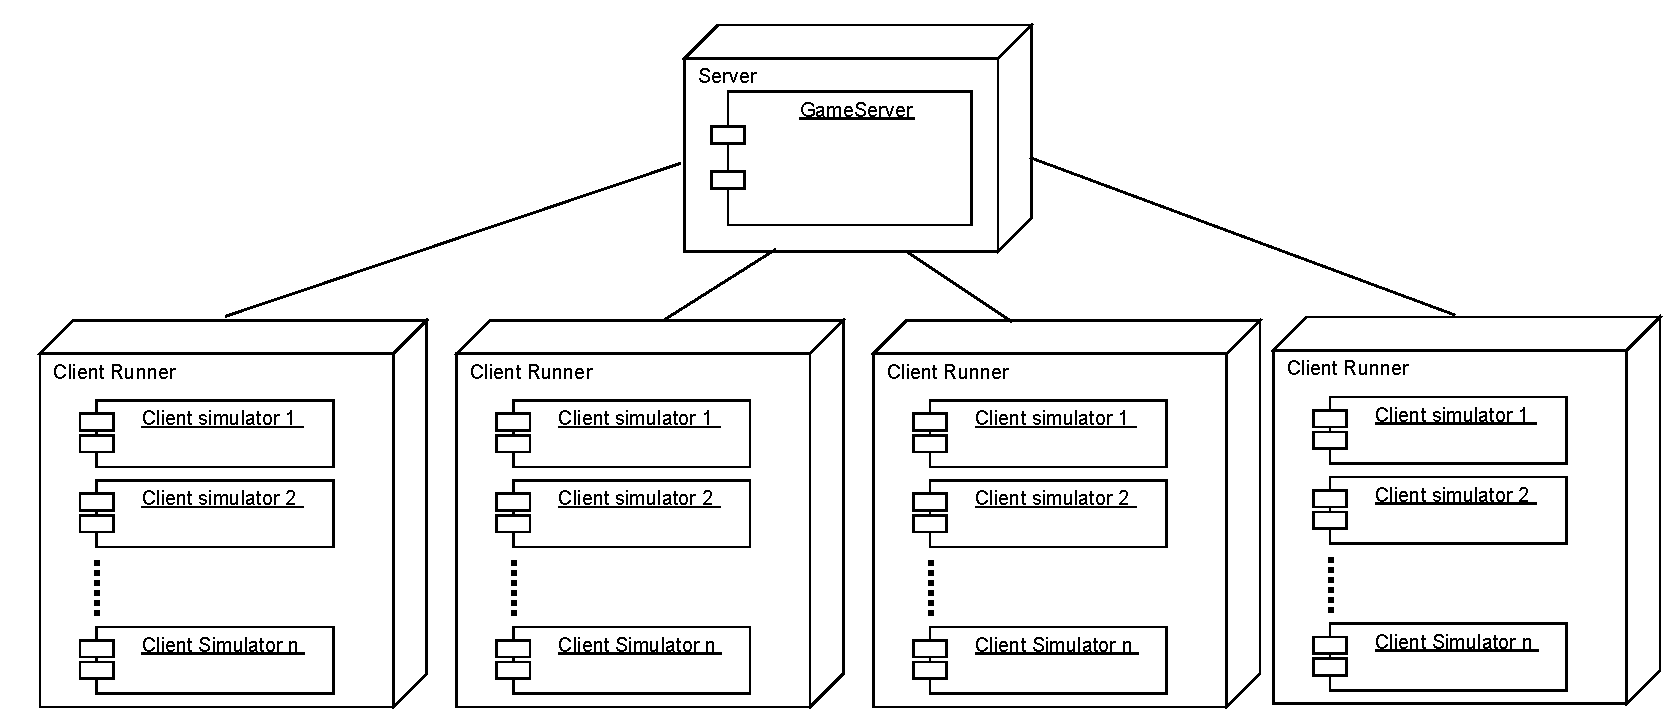
\includegraphics[width=1.0\linewidth]{FIG/DeploymentDiagram.pdf} 
%%   \caption{The
%%     experiments run on one server, with simulated players across multiple machines.}
%\end{figure}
  
To have a realistic behavior of the game clients, the game was run
with 5 human players playing the game with a game update frequency of
10~Hz. The network input to the server from this session was recorded
with a timestamp for each message. The recorded game interactions were
then played back multiple times in parallel to simulate a large number
of clients. To ensure that client performance is not a bottleneck, the
simulated clients were distributed among multiple physical
machines. Furthermore, as an average client generates 2.6~kbps network
traffic, the 1~Gbps local network interface that was used for the
experiments did not limit the performance. The game server was run on a
server machine containing 4 Dual-Core AMD Opteron 8218 (2600~MHz) with
16~GB RAM. To ensure comparable numbers, the server was taken down
between each test run.

\subsection{Response latency}
%
%
%\PH{I think we talked about several ways of discussing latency with different
%types of plots!? I do still think you should include several. One CDF (for a
%given number of clients) that looks at the average response time (not deadline
%misses), and then discuss different latency requirements from this (including
%the corresponding number of deadline missed in the given case) (the different
%latency requirements should be cited to be relevant). Then, a boxplot for each
%number of clients would be good - to show how the the latency changes with the
%number of users. When you reach problems - try to identify what causes the
%problems. }

\begin{figure*}[!t!] 
  \centering
  \vspace{-3mm}
  \subfigure[Single-threaded server]{
    \psfig{file=FIG/boxplot_st.eps, width=6.5cm,angle=-90}
    \label{fig:boxplot_st} 
  }
  \subfigure[Multi-threaded server]{
    \psfig{file=FIG/boxplot_mt.eps,width=6.5cm,angle=-90}
    \label{fig:boxplot_mt}
  }
  \caption{Response time for single- and multi-threaded servers
 (dotted line is the 100~ms threshold). }
  \label{fig:boxPlots}
\end{figure*}

The experiments were run with client numbers ranging from 40 to 800 in
increments of 40, where the goal is to keep the latencies below the
100~ms QoE threshold for FPS games~\cite{claypool++-2006}. Figure
\ref{fig:boxPlots} shows a box-plot of the response time statistics
from these experiments. All experiments used a pool of 48 worker
threads and distributed the network connections across 8 IP ports.

From these plots, we can see that the single-threaded implementation
is struggling to support 280 players at an average latency below
100~ms. The median response time is 299~ms, and it already has
extreme values all the way to 860~ms, exceeding the threshold for a good
QoE. The multi-threaded server, on the other hand, is handling the
players well up to 640 players where we are getting samples above 1
second, and the median is at 149~ms.

These statistics are somewhat influenced by the fact that the number of
samples is proportional to the update frequency. This means that long
update cycles to a certain degree get artificially lower weight.

\begin{figure}[t!]
  \centering 
  \subfigure[400 concurrent clients]{
    \psfig{file=FIG/cdf-400.eps, width=3cm,angle=-90}
    \label{fig:cdf-400}
  }
  \subfigure[800 concurrent clients]{
    \psfig{file=FIG/cdf-800.eps, width=3cm,angle=-90}
    \label{fig:cdf-800}
  } 
  \vspace{-3mm}
  \caption{CDF of response time for single-  and multi-threaded
    servers with 400 and 800 concurrent clients.}
  \label{fig:CDFPlots}
\end{figure}

Figure \ref{fig:CDFPlots} shows details of two interesting cases. In
figure \ref{fig:cdf-400}, the single-threaded server is missing all
its deadlines with 400 concurrent players, while the multi-threaded
version is processing almost everything on time. At 800 players
(figure~\ref{fig:cdf-800}), the outliers are going much further for
both cases. Here, even the multi-threaded implementation is struggling
to keep up, though it is still handling the load significantly better
than the single-threaded version, which is generally completely
unplayable.
%\vspace{4mm}
\subsection{Resource consumption}

\begin{figure}
  \centering %\vspace{-3mm}
  \psfig{file=FIG/cpu-load-620-mt.eps,angle=-90, width=8cm} %\vspace{-3mm}
  \caption{CPU load and response time for 620 concurrent clients on
    the multi-threaded server.}
  %\vspace{-3mm} 
  \label{fig:cpu-load-620}
\end{figure}

We have investigated the resource consumption when players connect to
the multhreaded server as shown in figure \ref{fig:cpu-load-620}. We
present the results for 620 players, as this is the highest number of
simultaneous players that server handles before significant
degradation in performance, as shown in figure
\ref{fig:boxplot_mt}. The mean response time is 133~ms, above the
ideal delay of 100~ms. Still, the server is able to keep the update
rate smooth, without significant spikes. The CPU utilization grows
while the clients are logging on, then stabilizes at an almost full
CPU utilization for the rest of the run. The two spikes in response
time happen while new players log in to the server at a very fast rate
(30 clients pr. second). Receiving a new player requires a lock in the
server, hence this operation is, to a certain degree, serial.

%#\PH{Nice to include this, but 1) we should have similar plots/results
%  for the single-threaded solution (a new line in the same plot?), 2)
%  cut the graph at 250 seconds - do not show the end with the dropping
%  load, and 3) why 620 clients (why not one where the average latency is below
%  100~ms for the multi-threaded solution -- maybe use 400 since this
%  har been shown in a plot before)?}
%\vspace{4mm}
\subsection{Effects of thread-pool size}

\begin{figure}
  \centering 
  \vspace{-3mm}
  \psfig{file=FIG/lineplot-threads.eps,angle=-90, width=8cm} %\vspace{-3mm}
  \caption{Response time for 700 concurrent clients on using varying number of threads. Shaded area from 5 to 95 percentiles.}
  \vspace{-3mm} 
  \label{fig:line-threads-700}
\end{figure}

To investigate the effects of the number of threads in the threadpool,
we performed an experiment where we kept the number of clients
constant while varying the number of threads in the pool. 700 clients
were chosen, as this number sligtly overloads the server. In
figure~\ref{fig:line-threads-700}, we see clearly that the system
utilizes more than 4 cores efficiently, as the 4 thread version shows
significantly higher response times. At one thread per core or more,
the numbers are relatively stable, with a tendency towards more
consistent low response times with more available threads, to about 40
threads. This could mean that threads are occasionally waiting for I/O
operations. Since thread pools are not preemptive, such situations
would lead to one core going idle if there are no other available
threads. Too many threads, on the other hand, could lead to excessive
context switch overhead. The results show that the average is slowly increasing after about 50 threads, though the 95-percentile is still decreasing with increased number of threads.

%\PH{Why the number 700? Use the same number of clients as in figure
%  5!? Can the plot have errorbars instead for the 5/95 percentiles
%  instead of a separate line (it is not intuitive how to read the
%  plot)?  The plot (ot at least the text) should also list the numbers
%for the single-threaded system!!!}

%\PH{Other things to evaluate? Workload per client? Background load? ...}

%% FW: QoE versus resources for reducing/increasing tick length 
%% What is the effect of network latency + server latency

\section{Discussion}
\label{sec:disc}

%\subsection {Spatial partitioning} \label{sec:spatialpartitioning}

Most approaches to multi-threaded game server implementations in the
literature (e.g., ~\cite{Abdelkhalek2004++}) use some form of
\textit{spatial partitioning} to lock parts of the game world while
allowing separate parts to run in parallel. Spatial partitioning is
also used in other situations to limit workload. The number of players
that game designers can allow in one area in a game server is limited
by the worst-case scenario. The worst case scenario for a spatially
partitioned game world is when everybody move to the same point, where
the spatial partitioning still ends up with everybody in the same
partition regardless of granularity. This paper investigates an
orthogonal and complementary approach which tries to increase the
maximum number of users in the worst case scenario where all players
can see each other at all times. Thus, spatial partitioning could be
added to further scale the game server.

%, as we want to investigate the worst case scenario, hence
%the numbers presented in this paper assume all players can see each
%other at all times. This means that the number of messages and
%interactions by necessity grows by the number of clients squared.
Experiments using multiple instances of a single-threaded server are not performed, as having clients distribueted acrosss multiple servers would mean partitioning the clients in areas where they can not interact, making numbers from such a scenario incomparable to the multithreaded solutions.
%
%\subsection{Limitations}

The LEARS approach does have \textit{limitations} and is for example not
suitable if the outcome of a message put restrictions on an object's
state. This is mainly a game design issue, but situations such as
trades can be accommodated by doing full transactions. 
The following
example where two players trade illustrates the problem: Player A
sends a message to player B where he proposes to buy her sword for X
units. After this is sent, player C steals player A's money, and
player A is unable to pay player B should the request go through. 
This is only a problem for trades \textit{within} a single game tick
where the result of a message to another object puts a constraint on
the original sender, and can be solved by means such as putting the
money in escrow until the trade has been resolved, or by doing a
transaction outside of LEARS (such as in a database).
%
Moreover, the design also adds some overhead in that the code is
somewhat more complex, i.e., all communication between elements in the
system needs to go through message queues. The same issue will also
create some runtime overhead, but our results still demonstrate a
significant benefit in terms of the supported number of clients.

Tasks in a thread pool can not be pre-empted, but the threads used for execution can. This distinction creates an interesting look into the performance trade-off of pre-emption. If the number of threads in the threadpool is equal to the number of CPU cores, we have a fully cooperative multitasking system. Increasing the number of threads allow for more pre-emption, but introduces context-switching overhead.
%\PH{Can the approach taken be ALSO be discussed in the context of the
%  keywords given in the CfP ? E.g., How do we use/schedule/utilize the
%  resources of a server compared to existing work?}

\section{Related Work}\label{sec:related}
At Netgames 2011~\cite{raaen++2011}, we presented a demo with a preliminary version of LEARS.
%
Significant research has been done on how to optimize game server
architectures for online games, both MMOGs and smaller-scale games. In
this section, we summarize some of the most important findings from
related research in this field. 
%
For example, "Red Dwarf", the community-based successor to "Project
Darkstar" by Sun Microsystems~\cite{waldo-2008}, is a good example 
of a parallel approach to game server design. Here, response time is 
considered one of the most important metrics for game server performance, 
and suggests a parallel approach for scaling. The described system 
uses transactions for all updates to world state, including player 
position. This differs from LEARS, which investigates the case for common actions where atomicity of transactions is not necessary. 

Work has also been done on scaling games by looking at the
optimization as a data management problem. The authors
in~\cite{white-2007} have developed a highly expressive scripting
language called SGL that provides game developers a data-driven AI
scheme for non-player characters. By using query processing and
indexing techniques, they can efficiently scale to a large number of
non-player objects in games. This group also introduces the concept \textit{state-effect pattern} in \cite{white++2008}, which we extend in this paper. They test this and other parallel concepts using a simulated actor interaction model, in contrast to this paper which evaluates a running prototype of a working games under realistic conditions.

%
Moreover, Cai et al.~\cite{Cai2002++} present a scalable architecture
for supporting large-scale interactive Internet games. Their approach
divides the game world into multiple partitions and assigns each
partition to a server. The issues with this solution is that the
architecture of the game server is still a limiting factor in worst
case scenarios as only a limited number of players can interact in the
same server partition at a given time. 
%
There have also been proposed
several middleware systems for automatically distributing the game
state among several participants. In~\cite{Glinka2007++}, the authors
present a middleware which allows game developers to create
large, seamless virtual worlds and to migrate zones between
servers. This approach does, however, not solve the challenge of many
players that want to interact in a popular
area. 
The research presented in~\cite{Muller2007++} shows that proxy
servers are needed to scale the number of players in the game, while the authors discuss the possibility of
using grids as servers for MMOGs. Beskow et al.~\cite{Beskow2009++} have also been
investigating partitioning and migration of game servers. Their
approach uses core selection algorithms to locate the most optimal
server.
We have worked on how to reduce latency by
modifying the TCP protocol to better support time-dependent
applications~\cite{Petlund2009}.  However, the latency is not only
determined by the network, but also the response time for the game
servers. If the servers have a too large workload, the latency will
suffer.

In~\cite{Abdelkhalek2003++}, the authors are discussing the behavior
and performance of multi-player game servers. They find that in the
terms of benchmarking methodology, game servers are very different
from other scientific workloads. Most of the sequentially implemented
game servers can only support a limited numbers of players, and the
bottlenecks in the servers are both game-related and
network-related. The authors in ~\cite{Abdelkhalek2004++} extend their
work and use the computer game Quake to study the behavior of the game. When
running on a server with up to eight processing cores the game suffers
because of lock synchronization during request processing. High wait
times due to workload imbalances at global synchronization points are
also a challenge.

A large body of research exits on
how to partition the server and scale the number of players by
offloading to several servers.  Modern game servers have also been
parallelized to scale with more processors. However, a large amount of
processing time is still wasted on lock synchronization, or the scaling is limited by partitioning requirements. In our game
server design, we provide a complementary solution and try to
eliminate the global synchronization points and locks, i.e., making the
game server ``embarrassingly parallel'' which aims at
increasing the number of concurrent users per machine.


\section{Conclusion}
\label{sec:conclusion} 

In this paper, we have shown that game servers can scale well with the
number of cores on a unified memory multi-processor system, even in
the case where all players must be aware of all other players and
their actions. The thread pool system balances load well between the
cores, and its queue-based nature means that no task is starved unless
the entire system lacks resources. Message passing through the
blocking queue allows objects to communicate intensively without
blocking each other. Running our prototype game, we show that the
8-core server can handle a factor of 2 more clients before the
response time becomes unacceptable.


From the research described in this paper, a series of further
experiments present themselves.
%
The relationship between linearly scaling load and quadratic load can
be tweaked in our implementation. This could answer questions about
which type of load scale better under multi-threaded implementations.
%
Another direction this work could be extended is to go beyond the
single shared memory computer used and distribute the workload
across clusters of computers. This could be achieved by implementing
cross-server communication directly in the server code, or by using
existing technology that makes cluster behave like shared memory
machines. 
%
Furthermore, all experiments described here were run with an update frequency of
10~Hz. This is good for many types of games, but different frequencies
are relevant for different games. Investigating the effects of running
with a higher or lower frequency of updates on server performance
could yield interesting results.
%
If, during the implementation of a complex game, it is shown that some
state changes must be atomic to keep the game state consistent, the
message passing nature of this implementation means that we can use
read-write-locks for any required blocking. If such cases are found
investigating how read-write-locking influence performance would be
worthwhile.
%
%Looking at the scope of garbage-collected languages, investigating how
%different garbage collectors compare for this system would be
%interesting. Investigating the newer multithreaded garbage collectors
%would be particularly interesting. Will they make the garbage
%collection overhead more manageable?  This naturally leads to the
%question of how the system will work without any garbage collection,
%by comparing the current Java implementation with a system written in
%a language with manual memory management, preferably C++.


%% IF ACCEPTED, ADD ACKNOWLEDGEMENT FOR THE CAMERA READY VERSION
%\section*{Acknowledgements}
%\noindent
%This work has been performed in the context of the  \textit{iAD} centre for
%Research-based Innovation (project number 174867) funded by the
%Norwegian Research Council.
%% Kjetil: Insert NITH in acknowledgements if needed.

\bibliographystyle{abbrv}
\bibliography{all}

\end{document}

